\documentclass[aspectratio=169]{beamer}
\usepackage[utf8]{inputenc}
\usepackage{amsmath}
\usepackage{tikz}
\usepackage{opensans}

\title{Sets}
\author{Paulo Fagandini}
\institute{NOVA School of Business and Economics}
\date{}

\institute{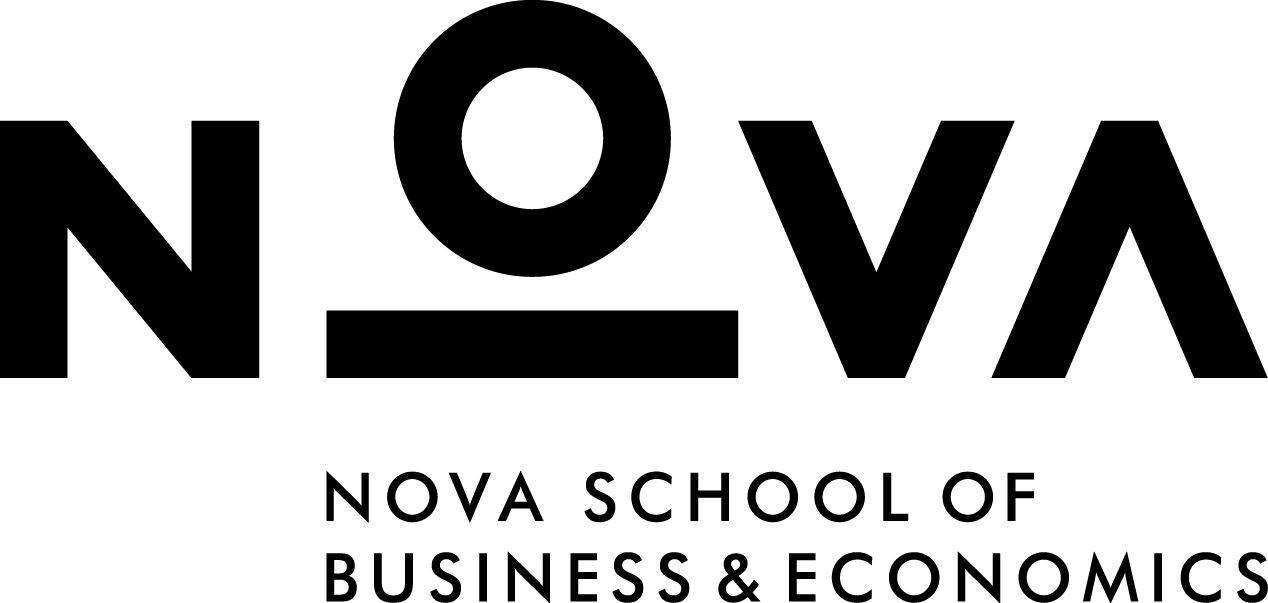
\includegraphics[scale=0.3]{NovaPrincipalV1.png}}
\date{}

\makeatletter
\setbeamertemplate{theorem begin}{%
  \setbeamercolor{block title}{bg=white,fg=black}%
  \setbeamercolor{itemize item}{fg=black}%
  \setbeamercolor{itemize subitem}{fg=black}%
  \setbeamercolor{itemize subsubitem}{fg=black}%
  \setbeamercolor{enumerate item}{fg=black}%
  \setbeamercolor{enumerate subitem}{fg=black}%
  \setbeamercolor{enumerate subsubitem}{fg=black}%
  \begin{\inserttheoremblockenv}
    {%
      \textbf{\inserttheoremname}
      %\inserttheoremnumber
      \ifx\inserttheoremaddition\@empty\else\ \inserttheoremaddition\fi%
    }%
    \normalfont%
}

\setbeamertemplate{theorem end}{%
    \end{\inserttheoremblockenv}%
}

\setbeamercolor{block title}{bg=white,fg=black}%
\setbeamercolor{itemize item}{fg=black}%
\setbeamercolor{itemize subitem}{fg=black}%
\setbeamercolor{itemize subsubitem}{fg=black}%
\setbeamercolor{enumerate item}{fg=black}%
\setbeamercolor{enumerate subitem}{fg=black}%
\setbeamercolor{enumerate subsubitem}{fg=black}%

\makeatother

\newtheorem{defenition}{Definition}[section]
\newtheorem{proposition}{Conjecture}[section]

\AtBeginSection{\frame{\sectionpage}}

\setbeamertemplate{footline}{
    \hspace{0.05\textwidth}
    \raisebox{3ex}{\insertshortauthor{}}\hfill
    \raisebox{3ex}{\insertframenumber{}/\inserttotalframenumber} \hfill
    {\raisebox{3ex}{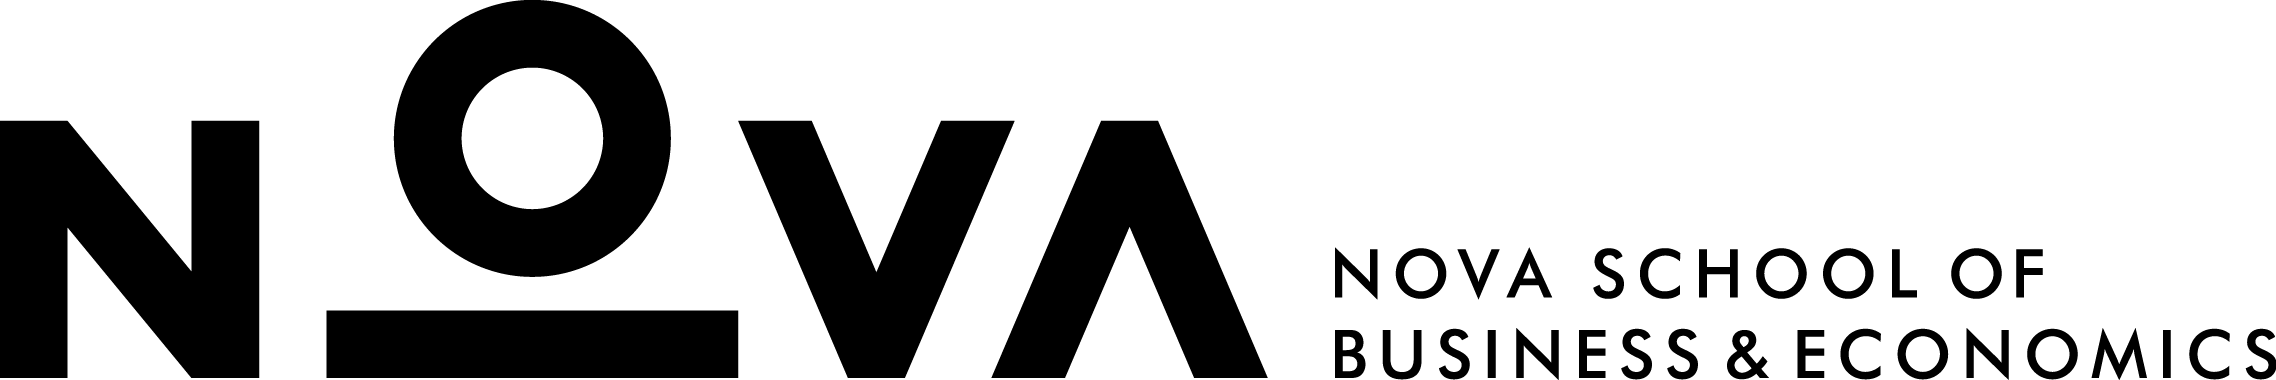
\includegraphics[height=0.04\textheight]{NovaPrincipalV2.png}}}
    \hspace{0.05\textwidth}
}

\setbeamertemplate{navigation symbols}{}

\setbeamercolor{title}{fg = black}
\setbeamercolor{subtitle}{fg = black}
\setbeamercolor{frametitle}{fg = white, bg = black}

\hypersetup{linkcolor=black, colorlinks=true}


\begin{document}

{
\setbeamertemplate{footline}{} 
\begin{frame}
  \titlepage
\end{frame}
}

\begin{frame}{Sets}

A \textbf{set} is a collection of \textbf{elements}. We say that element $a$ belongs to the set $A$, if $a$ is contained in $A$. We denote that: $a\in A$. If $a$ does not belong to $A$, we write $a\notin A$.\pause

\vspace{0.5cm}
There are two very important sets: The Universal set $\mathcal{U}$ and the empty set $\emptyset$.
    
\end{frame}

\begin{frame}{Sets}
    $\mathcal{U}$ is defined as the set that contains all the \emph{relevant} elements.
    
    \vspace{1cm}
    
    $\emptyset$ is defined as the set that does not contain any element.

    
\end{frame}

\begin{frame}{Sets}

    \begin{definition}
    Two sets $A$ and $B$ are said to be \textbf{equal} if $$\forall x,\quad x\in A\Leftrightarrow x\in  B$$
    \end{definition}

    \vspace{1cm}
    
    \begin{definition}
    
    $B$ is a \textbf{subset} ($\subseteq$) of $A$ if:
    
    $$\forall b\in B\Rightarrow b\in A$$
    \end{definition}
    
\end{frame}

\begin{frame}{Quick Quiz - 5 minutes}
    
    Show that if $A$ and $B$ are equal, then $A\subseteq B$ and $B\subseteq A$.
    
\end{frame}

\begin{frame}{Sets}
    \begin{definition}
        The \textbf{power} of a set is the set of all its subsets.
        $$\mathcal{P}(A):=\{B|B\subseteq A\}$$
    \end{definition}
    
    Note that the elements of $A$ do not belong to $\mathcal{P}(A)$, however, the sets containing a single element do. In other words the \textbf{set} $\{a\}$ is different than the \textbf{element} $a$.

    \begin{definition}
        The \textbf{cardinality} of a set is the number of elements it contains. It is denoted as $\#A$.
    \end{definition}

\end{frame}

\begin{frame}{Sets}
    Let's consider an example. Let $A=\{1,2,3\}$.
    
    \begin{itemize}
        \item $\mathcal{P}(A)=\{\emptyset, A,\{1\},\{2\},\{3\},\{1,2\},\{1,3\},\{2,3\}\}$.
        \item $\#A=3$, and $\#\mathcal{P}(A)=8$. 
    \end{itemize}
    
    In general, if $\#A$ is finite, then $\#\mathcal{P}(A)=2^{\#A}$.
\end{frame}

\begin{frame}{Sets}
    \begin{definition}
        A set $A$ is to be called finite, if $\#A$ is finite, and infinite otherwise.
    \end{definition}
    
    \vspace{0.5cm}
    
    Consider the set $\mathbb{N}$, the natural numbers. $\#\mathbb{N}=\infty$. This infinite set is special, because you can count it, from zero to infinity. We call this cardinality \emph{aleph zero}, $\aleph_0$, and the set is \textbf{countable}.
    
    \vspace{0.5cm}
    
    Now consider the set $\mathbb{R}$, which you know as the real numbers. Again, $\#\mathbb{R}=\infty$. This cardinal is called \emph{continuum}, and denoted with $c$. The sets with this cardinality are considered \textbf{uncountable}.
\end{frame}

\begin{frame}{Quick Quiz - 5 minutes}

Classify the cardinality of the following sets:
\begin{center}
\begin{tabular}{c|c}
    Set & Cardinality \\
    \hline
    $\mathbb{Z}$ &  \\
    $\mathbb{Q}$ &  \\
    $f(x) = a + bx, x\in\mathbb{R^+}$ &
\end{tabular}
\end{center}

\end{frame}

\begin{frame}{Quick Quiz - 5 minutes}

Classify the cardinality of the following sets:
\begin{center}
\begin{tabular}{c|c}
    Set & Cardinality \\
    \hline
    $\mathbb{Z}$ & $\aleph_0$  \\
    $\mathbb{Q}$ & \\
    $f(x) = a + bx, x\in\mathbb{R^+}$ &
\end{tabular}
\end{center}

\end{frame}

\begin{frame}{Quick Quiz - 5 minutes}

Classify the cardinality of the following sets:
\begin{center}
\begin{tabular}{c|c}
    Set & Cardinality \\
    \hline
    $\mathbb{Z}$ & $\aleph_0$  \\
    $\mathbb{Q}$ &  $\aleph_0$ \\
    $f(x) = a + bx, x\in\mathbb{R^+}$ &
\end{tabular}
\end{center}

\end{frame}

\begin{frame}{Quick Quiz - 5 minutes}

Classify the cardinality of the following sets:
\begin{center}
\begin{tabular}{c|c}
    Set & Cardinality \\
    \hline
    $\mathbb{Z}$ & $\aleph_0$  \\
    $\mathbb{Q}$ &  $\aleph_0$ \\
    $f(x) = a + bx, x\in\mathbb{R^+}$ & $c$
\end{tabular}
\end{center}
\end{frame}

\begin{frame}{Sets}
    \begin{definition}
        Consider $A$ and $B$ to be subsets of $\mathcal{U}$.
        \begin{enumerate}
            \item The union between $A$ and $B$: $$A\cup B:=\{c|\quad c\in A \quad\vee\quad c\in B\}$$
            \item The intersection between $A$ and $B$: $$A\cap B:=\{c|\quad c\in A \quad\wedge\quad c\in B\}$$
            \item The difference between $A$ and $B$:$$A\setminus B:=\{c|\quad c\in A \quad \wedge \quad c\notin B\}$$
            \item The complement of $A$, $$A^c:=\mathcal{U}\setminus A$$ 
        \end{enumerate}
    \end{definition}
\end{frame}

\begin{frame}{Sets}
    
    If two sets ($A$ and $B$) are such that there is a valid operation between their elements, say ``$ope$'', then:
    
    $$A \quad ope \quad B:=\{c|c= a\quad ope \quad b,\quad a\in A \quad b\in B\}$$
    
    Example: $A=\{1,2\}$, $B=\{3,4,7\}$,
    \begin{itemize}
        \item $A+B=\{4,5,6,8,9\}$
        \item $A-B=\{-6,-5,-3,-2,-1\}$
    \end{itemize}
    
\end{frame}

\begin{frame}{Sets}
    \begin{definition}
    $A$ and $B$ are \textbf{disjoint} if $$A\cap B=\emptyset$$
    \end{definition}
    
    \begin{definition}
    
    A \textbf{partition} $P$ of a set $A$, is a set of $k$ nonempty subsets of $A$, $\{A_i\}_{i=1}^{k}$, such that:
    
    \begin{itemize}
        \item $A_i$ and $A_j$ are disjoint for any $i\neq j$.
        \item $\bigcup_{i=1}^{n}A_i=A$
    \end{itemize}
    
    
    \end{definition}
    
\end{frame}
\begin{frame}{Sets}
    \begin{definition}
    Let $a\in A$, and $b\in B$ (nothing prevents $A$ being equal to $B$), the \textbf{ordered pair} $(a,b)$ is defined as:
    
    $$(a,b):=\{a,\{a,b\}\}$$
    
    \end{definition}
    
    Note that while $\{a,b\}=\{b,a\}$ (both sets have the same elements), $(a,b)\neq(b,a)$.
\end{frame}

\begin{frame}{Sets}
    \begin{definition}
    The \textbf{product} of two sets is defined as:
    
    $$A\times B:=\{(a,b)| a\in A\quad b\in B\}$$
    \end{definition}
    
    \begin{definition}
        The ordered \textbf{n-tuple} of $A$ is:
        
        $$A^n := \underbrace{A\times A\times A \times\ldots\times A}_{\text{n times}}$$
    \end{definition}
\end{frame}

\begin{frame}{Numbers and Sets}
    \begin{itemize}
        \item The naturals, $\mathbb{N}:=\{0,1,2,3,\ldots\}$
        \item The integers, $\mathbb{Z}:=\{\ldots,-2,-1,0,1,2,\ldots\}$
        \item The rationals, $\mathbb{Q}:=\left\{\frac{p}{q}|p\in\mathbb{Z},q\in\mathbb{Z}\setminus\{0\}\right\}$
        \item The reals, $\mathbb{R}:=\mathbb{Q}\cup I$, with $I$ being the irrationals.
    \end{itemize}
    
    It holds that $$\mathbb{N}\subseteq\mathbb{Z}\subseteq\mathbb{Q}\subseteq\mathbb{R}$$
    
\end{frame}

\begin{frame}{Working on the Real Numbers}

Let $a<b$, and $a,b\in \mathbb{R}$.

\begin{enumerate}
    \item $[a,b]$ is called closed interval. This set contains all the real numbers between $a$ and $b$, with $a$ and $b$ included.
    \item $(a,b]:=[a,b]\setminus\{a\}$.
    \item $[a,b):=[a,b]\setminus\{b\}$.
    \item $(a,b):=[a,b]\setminus\{a,b\}$. This is called an open interval. It is also the \emph{interior} of $[a,b]$.
\end{enumerate}
    
\end{frame}

\begin{frame}{Working on the Real Numbers}
    If a subset A of $\mathbb{R}$ is such that $A:=\{x\in\mathbb{R}|x\leq a\}$ we can write it as $(-\infty,a]$.
    
    \vspace{1cm}
    
    The side where the $\infty$ is, is always ``open''.
\end{frame}

\begin{frame}{Working on the Real Numbers}
    \begin{definition}
        Let $x\in\mathbb{R}$, the module of $x$ is,
        
        \begin{eqnarray*}
            |x|=\left\{
                \begin{array}{c}
                   x \quad \text{if} \quad x\geq 0\\
                  -x \quad \text{otherwise}
            \end{array}
            \right.
        \end{eqnarray*}
    \end{definition}

\end{frame}

\begin{frame}{Working on the Real Numbers}
    \begin{definition}
        Let $A\subseteq\mathbb{R}$,
        \begin{enumerate}
            \item $A$ is said to be bounded from above if $$\exists M\in\mathbb{R}\quad s.th.\quad \forall a\in A, a\leq M$$ $M$ is an upper bound of $A$.
            \item $A$ is said to be bounded from below if $$\exists M\in\mathbb{R}\quad s.th.\quad \forall a\in A, a\geq M$$ $M$ is a lower bound of $A$.
            \item $A$ is said to be bounded if it is bounded from above and from below.
        \end{enumerate}
    \end{definition}
\end{frame}

\begin{frame}{Working on the Real Numbers}
    Let $A\subseteq\mathbb{R}$ be bounded.
    
    \begin{definition}
        \begin{itemize}
            \item The \textbf{supremum} of A ($sup(A)$) is the lowest of its upper bounds.
            \item The \textbf{infimum} of A ($inf(A)$) is the highest of its lower bounds.
        \end{itemize}
    \end{definition}
    
    If $sup(A)\in A$, it is called the \textbf{maximum} of $A$ ($max(A)$).
    
    If $inf(A)\in A$, it is called the \textbf{minimum} of $A$ ($min(A)$).
\end{frame}
\end{document}
